\chapter{Construction of the Survey}
\label{chp:amtsurvey} 

To be able to map to what extent people care, and are aware, of their Facebook settings, regarding privacy, security and interdependent privacy, we designed and distributed a survey. The complete survey can be found in Appendix \ref{chp:appendixA}. The survey addressed the different settings available on Facebook, and awareness regarding Facebook applications and knowledge about interdependent privacy. For the design of the survey we utilized SurveyMonkey, which provide a web-based survey solution (see section \ref{sec:sm}). We distributed the survey on two platforms, namely Amazon Mechanical Turk (MTurk) and Facebook. Amazon Mechanical Turk is a Internet marketplace where human intelligence is utilized to perform various tasks \cite{amazonweb}. For more information about Amazon Mechanical Turk, see section \ref{sec:amt}. To reach out to an even larger audience, we also posted the survey-link on our private Facebook pages. In this chapter we will describe how we designed the survey, and how it was structured, and how we distributed our survey.


\subsubsection{Constructing the Survey.}
There is not much research on the area of interdependent privacy. When designing the questions to our survey, we wanted to be able to create an image of people's Facebook usage, how they set their settings, how much they knew and cared about their privacy, and to what extent their privacy was dependent on other users. We quickly chose to use MTurk as a platform for distributing the survey, because we wanted to create an image of the average Facebook user, as well as getting a high diversity among the respondents (different countries, age, education etc.). Previous research shows positive results with the use of MTurk \cite{expectations,incentivesAmt}. 

\paragraph{}
We started implementing the survey inside the survey template provided by MTurk, but after some consideration, we found that MTurk did not fulfil our requirements for design. We therefore chose to implement the survey using SurveyMonkey instead. During the creation of the survey, we thought that it would be better to include some extra questions, rather than leaving some out. This was to assure that we got all the information we would need in order to perform our analysis. When the survey first was distributed, we were no longer able to edit the questions. We therefore chose to include questions, not only regarding privacy and interdependent privacy, but also other aspects of Facebook usage. Like for instance some questions about security settings, usage, personal experience in regard to photos and comment sharing.

\section{Design}
MTurk offers a template for creating surveys, and this template uses HTML-code. It is simple, but requires more work and knowledge from the requester. We found the template to not be very user friendly, and it did not offer many design options. Our survey consisted of many questions, and some of them had follow-up questions requiring text answers. It was then desirable to separate these into two different pages, as we did not want the respondents to have their answers affected by the next question. It required more of the respondent to write a text answer, so to avoid them answering based on the next question we separated the questions onto different pages. For example, we had one question asking whether or not the use of Facebook has lead to any uncomfortable situations. If the user answered "Yes", a follow-up question asking to describe the situation that occurred would appear. If the user answered "No" the follow-up question would be skipped. If the user had seen the follow-up question, he/she may not be bothered to answer yes even though this may have been the truthful answer. We did not find an easy solution to implement this design feature in MTurk, so we looked for other options. In addition to providing their own "Survey"-template, MTurk also provides a "Survey Link"-template. This means that you can create the survey somewhere else, and link to it in MTurk. We chose the latter, and used SurveyMonkey to create our survey. SurveyMonkey provided us with the tools and features necessary to design our survey as desired. 

\subsubsection{Features we used in SurveyMonkey.}
SurveyMonkey offers several features, and has an intuitive and simple user interface. It was easy to implement the questions, and separate them into different pages, which was of high value to us. SurveyMonkey offers the ability to customize the appearance (color/theme, layout, etc.) of the survey to a higher extent than MTurk. We included a picture of the university logo, to emphasize the seriousness of the survey, as shown in \fref{fig:frontpage}. SurveyMonkey also offers many different types of question forms, like multiple choice, text box, matrix and drop-down menus, and restrictions on the questions. Some of the restrictions that we used was to limit the amount of characters in the text boxes, to avoid too long answers. We also made almost all questions mandatory, meaning that the respondents had to answer them before being able to move on to the next question. As mentioned we divided the questions on to several different pages. In addition to the advantages already mentioned, it would also give the respondents the impression that the survey is shorter. Each page has a title at the top, grouping the different areas. A progress bar was added to the bottom, showing in percent how far into the survey the respondent was at any time. This gave a good overview, and the user got a feeling of how much was left of the survey. We chose to use these features to avoid overwhelming the respondents with too many questions at a time. 

SurveyMonkey offers a great user interface also when it comes to reviewing the answers. It is possible to see graphs showing the distribution of answers to all of the questions, as well as individual answers. SurveyMonkey also offers features as filtering and comparing, which made the analysis a lot easier, especially when having a large number of respondents. 

\section{Survey Structure} 

\begin{figure}[t]
\centering
\fbox{
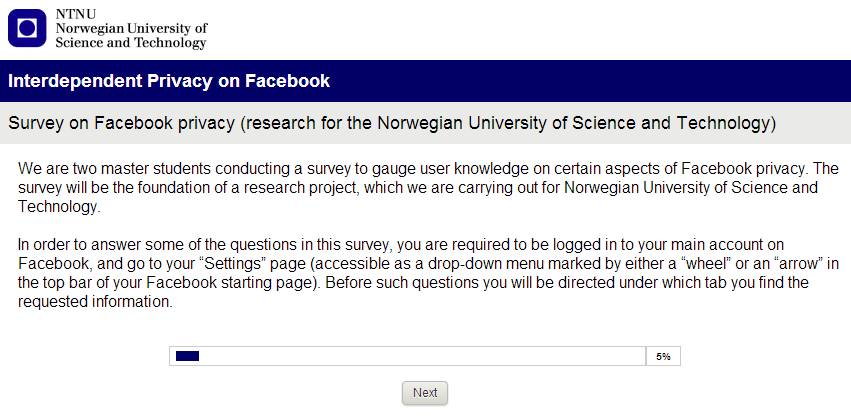
\includegraphics[width=1\textwidth]{firstpagesurvey.png} }
\caption[Front page of the survey]{\textbf{Front page of the survey.}} 
\label{fig:frontpage}
\end{figure}

The first page seen when taking the survey, was an introduction page that shortly explained what the survey was about, and its purpose. This page emphasized the seriousness of the survey. When people saw that it was a research survey carried out by master students at an university, we believed people would answer in a serious manner. The front page also included the requirements for taking the survey, and a short explanation on where to find answers requested in some of the questions. This is shown in \fref{fig:frontpage}. As mentioned earlier, we divided the questions into different areas, and we will now go through each area emphasizing and elaborating the questions we considered most relevant and important. 
 

\subsection{Facebook Usage}
Following the first page, was a single page about Facebook usage. This page included questions about sign-up year, how often they checked their Facebook page, and number of friends. 

\subsection{Facebook Privacy: Settings}
This was a part of the survey where the users needed to be logged into their main account on Facebook in order to check how their privacy settings looked. The questions were taken directly from the "Privacy"-settings and "Timeline and tagging"-settings on Facebook. We divided these questions on to 4 different pages. Before we started asking about specific settings, we asked the users how often they had checked their Facebook privacy settings during the last year. The following pages asked for the privacy settings, and the other for the timeline and tagging settings. These questions were straightforward for the user, since all they had to do was to render the settings they had set themselves. This would easily show us how many of the survey participants that actually had checked their settings, and to what extent they had made them more, or less, private than default. At the end we asked the users whether or not they considered changing their settings after having reviewed them. This could make for some interesting observations, and could also give an impression of whether or not the users cared or were aware of the settings. 

\begin{figure}[t]
\centering
\fbox{
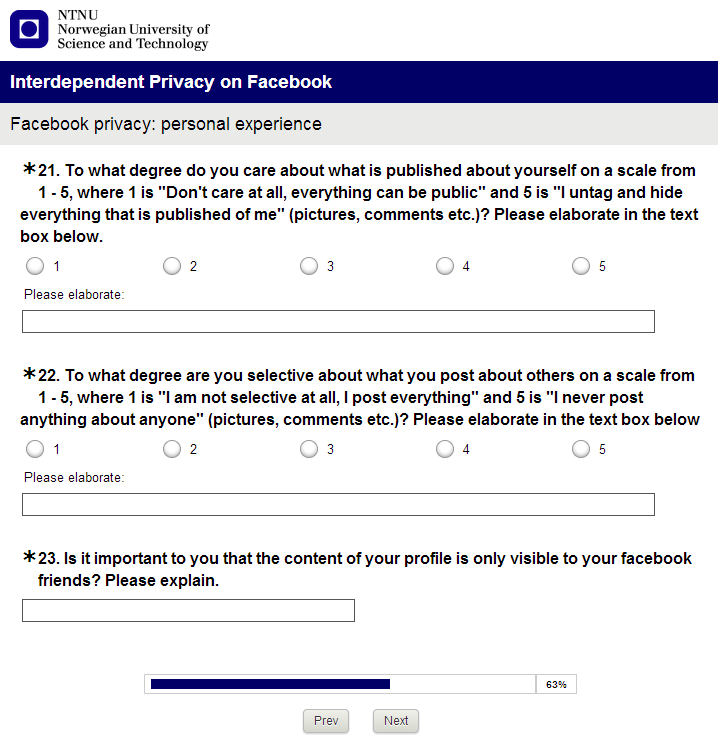
\includegraphics[width=1\textwidth]{page12.png} }
\caption[Question 21 and 22 in the survey concerning personal experience]{\textbf{Question 21 and 22 in the survey concerning personal experience.}} 
\label{fig:page12}
\end{figure}

\subsection{Facebook Privacy: Personal Experience}

This group of questions focused on the users' personal experience with concern to both privacy and interdependent privacy. We asked whether or not the respondents had experienced that their use of Facebook had affected their professional life, or led to any uncomfortable situations. Both of these questions had a follow-up question where the users were asked to describe the situation that occurred. The user would only be sent to the page with the follow-up question if the user answered yes. If the user answered no, the page with the follow-up question would be skipped. 

A big part of Facebook consists of sharing photos and comments with others, we therefore asked the respondents to indicate on a scale from 1 to 5 how much they care about what was published about themselves, and what they publish about others, see \fref{fig:page12}. It was mandatory for the users to give an answer on the scale. We added a text box for the users to elaborate if desired, but this was voluntarily. We received a total of 250 responses on our survey, and 190 of them chose to elaborate. 

\subsection{Facebook Privacy: Apps}

\begin{figure}[t]
\centering
\fbox{
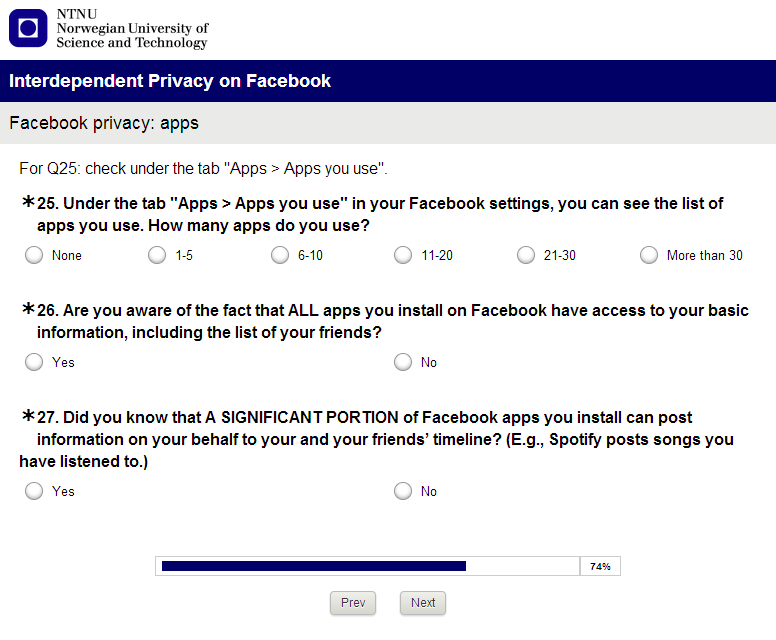
\includegraphics[width=1\textwidth]{page14.png} }
\caption[Question 25, 26 and 27 in the survey concerning Facebook apps]{\textbf{Question 25, 26 and 27 in the survey concerning Facebook apps.}} 
\label{fig:page14}
\end{figure}

\begin{figure}[t]
\centering
\fbox{
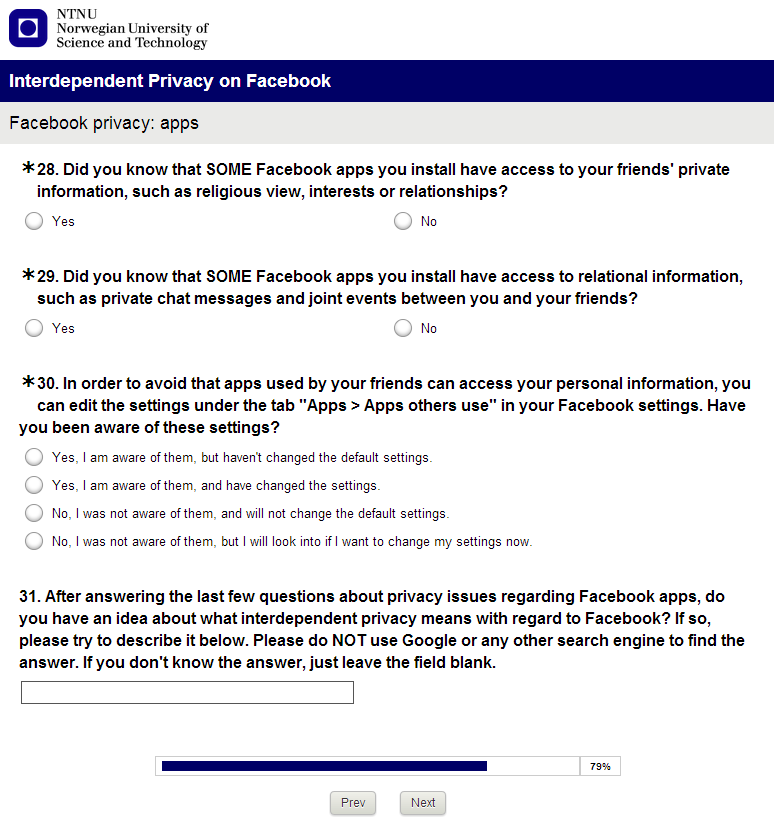
\includegraphics[width=1\textwidth]{page15.png} }
\caption[Question 28, 29, 30 and 31 in the survey concerning Facebook apps]{\textbf{Question 28, 29, 30 and 31 in the survey concerning Facebook apps.}} 
\label{fig:page15}
\end{figure}

This was the part of the survey that concerned interdependent privacy (see section \ref{sec:intpriv}), and also the most important part of our survey. As mentioned earlier, this is a relatively unknown term, so we wanted to find out whether or not the respondents knew the meaning of interdependent privacy. When installing an app on Facebook, it asks for the user's basic information, and often more information about the user and the user's friends. For more detailed information about the app-platform, see subsection \ref{subsec:app}. Question 26, 27, 28 and 29 (see \fref{fig:page14} and \fref{fig:page15}) asked about the user's awareness regarding what kind of information the apps could retrieve. There exists settings directed towards apps on Facebook (see \tref{tab:settings}). Question 25 concerned the number of apps the respondents use. Question 26, 27, 28 and 29 concerned the user's awareness connected to apps permission requests on Facebook. In question 30 (\fref{fig:page15}) we asked the user to look at one of the app settings, "Apps others use". In this setting the user can decide what information they want to make available to apps other people use, in other words, control the categories of information that people can bring with them when they use apps. We did not ask for more specifics about what information they share, because this was not relevant to our research. What was relevant was whether or not they knew it existed, and were aware of what kind of information they shared. We finished this part of the survey with the same question we started it with, if they knew the meaning of interdependent privacy. We wanted to ask again to see if they got a higher understanding of the term after answering questions about apps, and saw how it is all interconnected. 


\subsection{Facebook Security: Settings}
The main focus in this report is on privacy, not security. At the same time, we wanted to ask a few questions regarding Facebook security settings as well. The reason for this was that we wanted to see if there was a connection between strict security settings, and strict privacy settings among the respondents. The questions concerned whether or not the respondents used secure browsing and login notification.

\subsection{Demographics}
In the last part of our survey, we asked for demographic information about the respondents. This to get a hunch of what kind of people had taken the survey. We chose to put the demographics part at the end, rather than at the beginning. We assumed that a respondent's attention span would get lower during the survey, we therefore wanted to put the "easy" questions at the end, since they require less focus. These questions consisted of: gender, age, country, family situation, highest qualification/degree, employment status and income. Although these questions were easy to answer, they were very important to include. When analysing, they are necessary in order to draw comparisons between, for example, age and/or gender. An interesting factor will be to look at where the respondents using MTurk come from.  

\section{Distributing the Survey}


First we created a requester account on MTurk. We did this using an already existing Amazon account. While creating the project (our project contained only one HIT) we filled out the properties shown in \fref{fig:amtedit}. First we had to give a short title and description to describe our HIT to the workers. This is the information that is shown to the workers before they choose to accept, or skip, the HIT. We also had to decide a reward for the workers. We had limited time, and wanted our HIT to be as attractive as possible, and therefore chose to have a higher reward than average. We sat the reward to be \$1.5 per completed assignment. We estimated that it would take approximately 15 minutes to take the survey, and this would give an hourly wage of \$6. We were also asked to set a maximum number of assignments per HIT, this means number of unique answers. We sat this number to be 250. We felt that 250 responses would give us a very good foundation to base our analysis on. MTurk defines a feature that let the requester review the answers, and then choose to either approve or discard them. When discarding an answer, the worker would not get paid. If we did not manually approve the answers, they would automatically be approved after 3 days. We made the HIT available for only 21 days. To get a high quality on the responses, we were advised to use "Master Workers". This is users that have a good reputation from previous work done on MTurk. See section \ref{sec:methodology} for more information about "Master Workers". 

\begin{figure}[t]
\centering
\fbox{
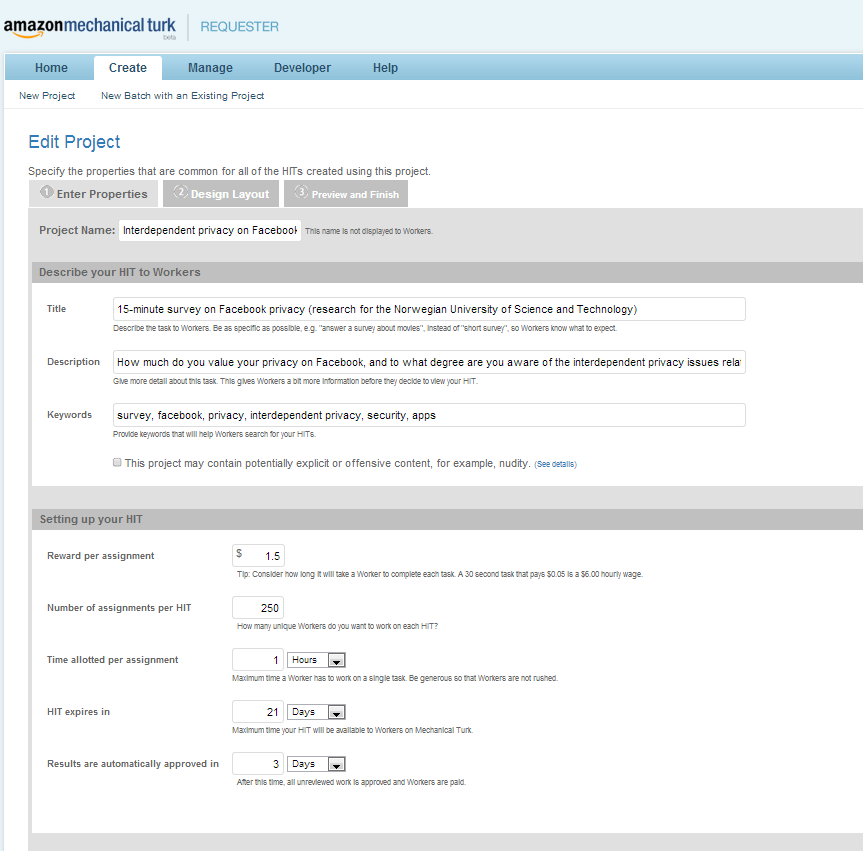
\includegraphics[width=1\textwidth]{amtedit.png} }
\caption[Layout for creating an MTurk project]{\textbf{Layout for creating an MTurk project.}} 
\label{fig:amtedit}
\end{figure}

\begin{figure}[t]
\centering
\fbox{
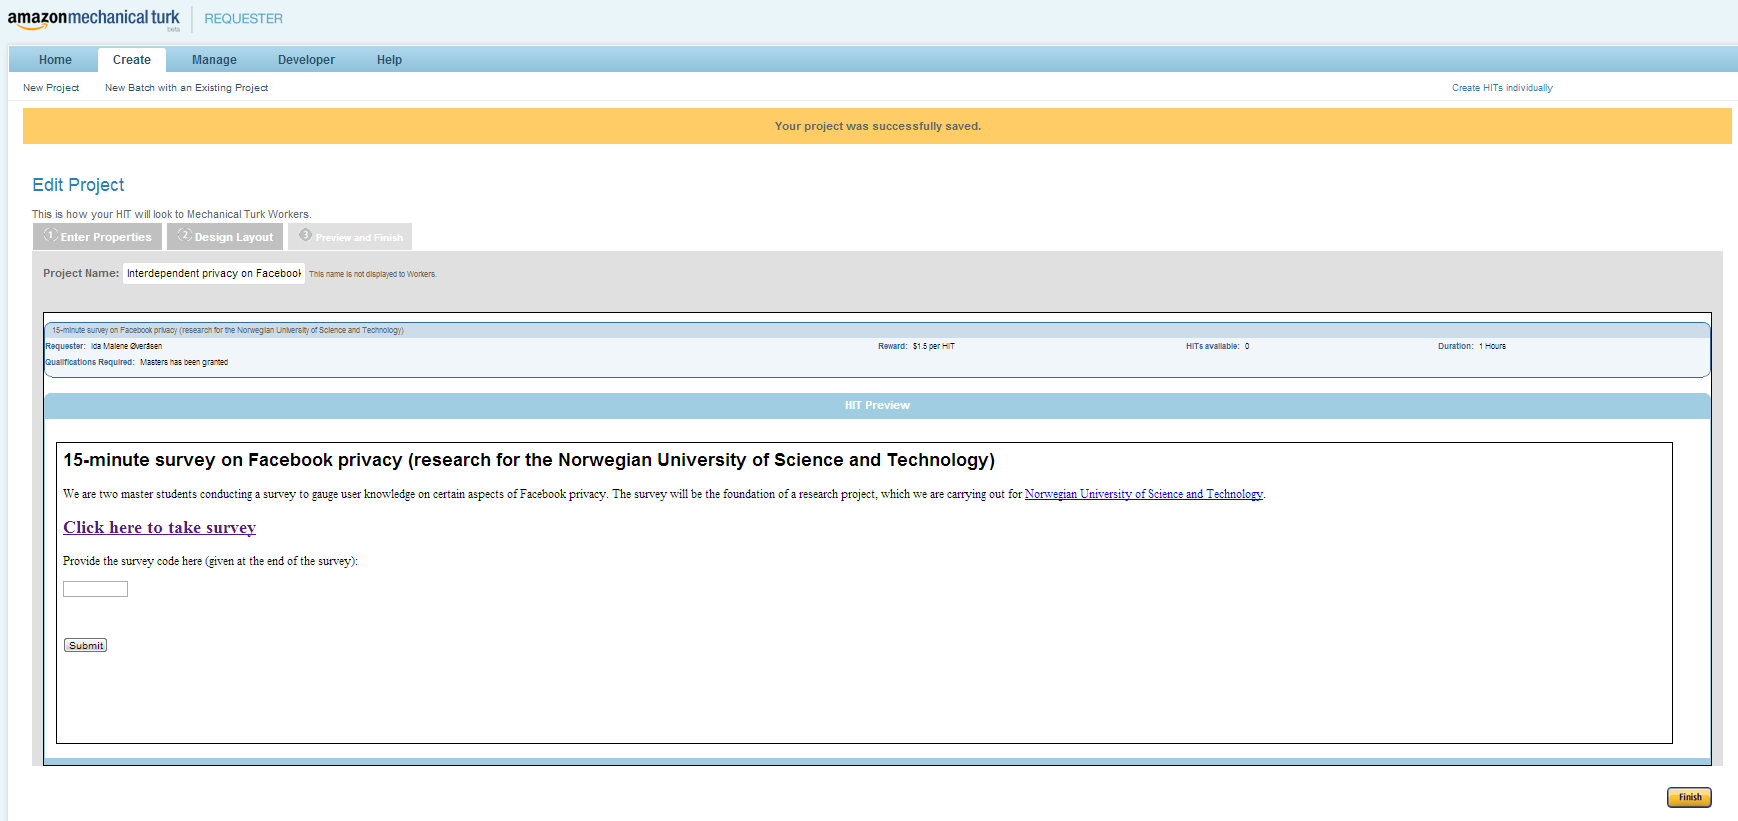
\includegraphics[width=1\textwidth]{amtlayout.png} }
\caption[The design and layout of the survey on MTurk]{\textbf{The design and layout of the survey on MTurk.}} 
\label{fig:amtlayout}
\end{figure}

Next we filled in the "Survey-Link"-template provided by MTurk, and the result of this is shown in \fref{fig:amtlayout}. It contains a title and a short description. In the description we linked to the homepage of the Norwegian University of Science and Technology, to emphasize the seriousness of the survey. In addition it contained the link to the survey on SurveyMonkey, as well as a field for the users to enter a survey code. This code was provided to them after completing the survey, and worked as an assurance for us, so we only paid the people who actually took the survey. To avoid workers cheating with the code (for example getting the code from a fellow MTurk-worker), we changed it several times during the survey's lifetime. 

\begin{figure}[t]
\centering
\fbox{
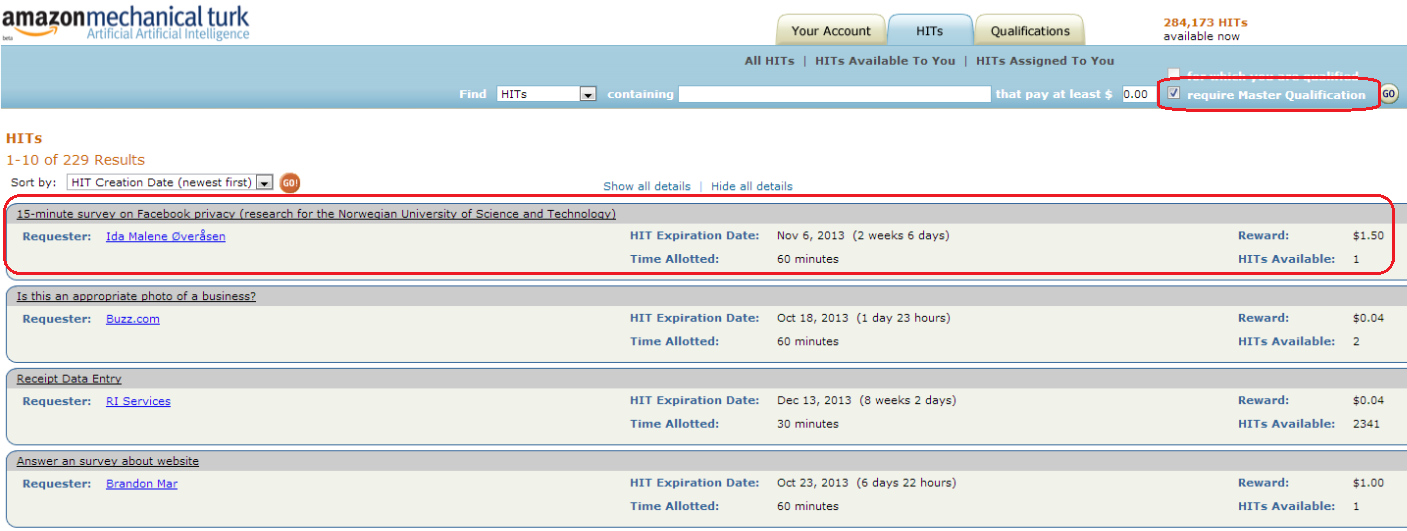
\includegraphics[width=1\textwidth]{hitisout.png} }
\caption[Our HIT is published]{\textbf{Our HIT is published.} This figure shows our HIT in the list of all HITs available that requires "Master Workers".} 
\label{fig:hitout}
\end{figure}

After editing the project, as described above, the HIT was ready to be published. The published HIT is shown in \fref{fig:hitout}. After filtering on HITs requiring "master" qualification, our HIT is shown at the top. 
Once our HIT was out, all we could do were to monitor it (approve or discard answers), and wait for people to respond. 

\begin{figure}[t]
\centering
\fbox{
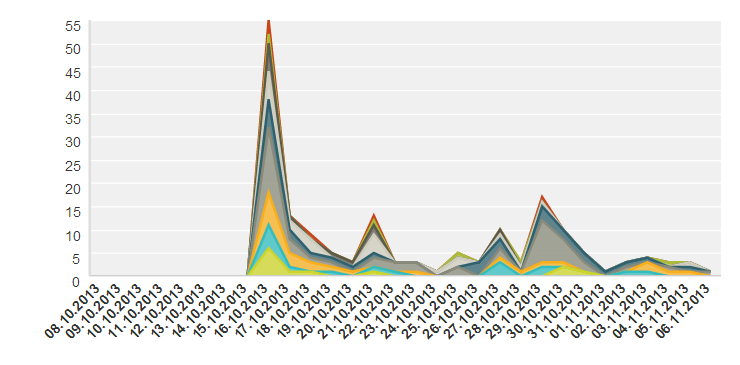
\includegraphics[width=1\textwidth]{answersamt.png} }
\caption[Daily distribution of number of answers from MTurk]{\textbf{Daily distribution of number of answers from MTurk.}} 
\label{fig:answersamt}
\end{figure}

\begin{figure}[t]
\centering
\fbox{
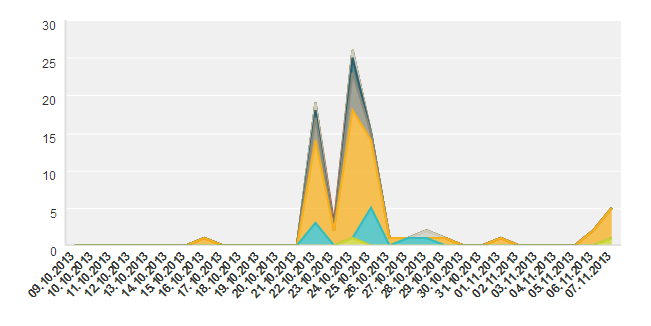
\includegraphics[width=1\textwidth]{answersfacebook.png} }
\caption[Daily distribution of number of answers from Facebook]{\textbf{Daily distribution of number of answers from Facebook.}} 
\label{fig:answersfacebook}
\end{figure}

We mainly wanted to distribute our survey on MTurk, to try it out as a research tool, and because of it's high diversity. But in addition to distributing the survey on MTurk, we decided to also share it with our friends on Facebook. We wanted to reach out to an even wider audience, as well as making our Facebook friends aware of their settings. Most of our Facebook friends mainly consist of fellow students, with high technical knowledge. We were hoping for at least 30 extra respondents as a result from our post on our private Facebook profiles. We received 77 respondents and were amazed with the outcome. A few times during the 3 weeks the survey was out, we pushed our post to the top of our friends' news feeds by commenting on it. Three of our friends even chose to share it on their own Facebook profile. This was probably one of the reasons why we got more answered than expected. We posted the survey on Facebook a few days later than the HIT was published on MTurk.  

\fref{fig:answersamt} and \fref{fig:answersfacebook} shows the daily distribution of number of answers, from MTurk and Facebook respectively. You can see from \fref{fig:answersamt} that we had the highest peak in responses the day it was published on MTurk, with 55 unique answers, and the second day it dropped to 13 answers. The number of responses varied during the rest of the period, as the figure shows. 

\section{Feedback on the Survey}
We got a lot of positive feedback on our survey from our Facebook friends. Many have "liked" it, and many have commented on it. The comments focused mainly on the eye opening aspects of the survey and that it was informative. Some said the survey made them clean-up their settings. Some mentioned that they believed they had good control over their settings, but after taking the survey they realized that this was not the case. Overall, the feedback was very positive. As mentioned above, three of our Facebook friends even chose to share the survey further, meaning that they were pleased with it and thought it was both good and informative. 

Our survey has also been mentioned in forums as, for example, mturkform.com and mturkgrind.com. Most of the comments regarding our survey on these forums were about the time consumed taking the survey and it's complexity. The comments from mturkforum was: \textit{"Time 5 min 35 sec - slow b/c I wanted to learn more about FB privacy..."} and \textit{"Took 8 minutes, light writing but very simple"}.
The comments from mturkgrind was: \textit{"About 5 minutes"} and \textit{"Took 8 minutes, very simple and probably could do it in less time. Light writing"}.





